\documentclass[main.tex]{subfiles}
\graphicspath{{\subfix{../images/}}}
\begin{document}



LEAVING AS EXAMPLE
Thus, the equation for the calibration curve is:
\begin{equation*}
    \mathcolorbox{Lavender}{A = 0.21066718C_{\text{digested}} -0.0077607}
\end{equation*}

A results and discussion section which integrates answers to the questions above, assignment of spectra, 
includes a discussion of yields and data collected. It is useful if you include subheadings etc to draw attention to 
the answers you provide to the questions.

As large volumes of data are generated or extensive calculations will be done, the results of these need 
to be presented in an appropriate style (graph, table or figure) and these results need to be described 
and discussed in the context of the experimental aims.

\subsection{Electron Transfer Kinetics via Emission Spectroscopy}
\subsubsection*{Results}
\begin{figure}[H]
    \centering
    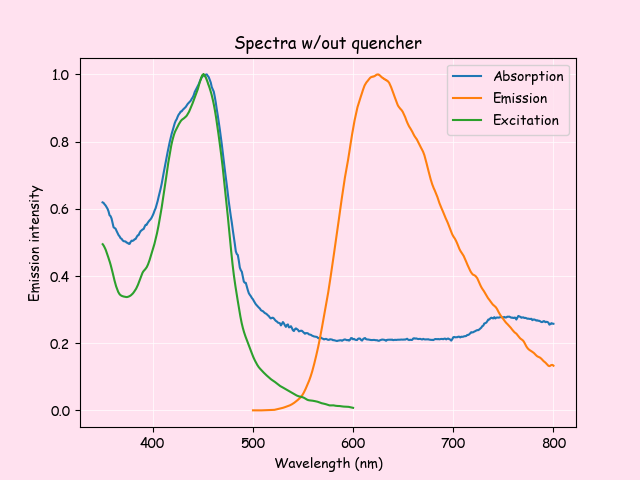
\includegraphics[width = 0.7\linewidth]{part1_noq.png}
    \caption{REDO TITLE}
    \label{fig:enter-label}
\end{figure}
\subsubsection*{In Class Analysis}
\textbf{Question 1} 
\begin{figure}[H]
     \centering
     \begin{subfigure}[b]{0.49\textwidth}
         \centering
         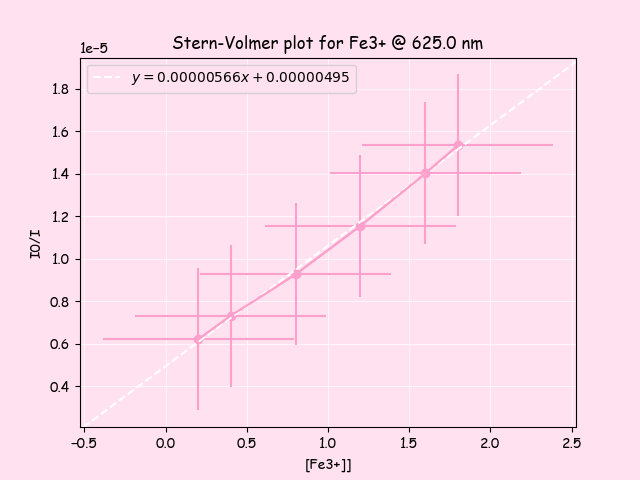
\includegraphics[width=\textwidth]{part1_q1_Fe.png}
         \caption{\ce{Fe^{3+}}}
         \label{fig:part1_q1_fe}
     \end{subfigure}
     \hfill
     \begin{subfigure}[b]{0.49\textwidth}
         \centering
         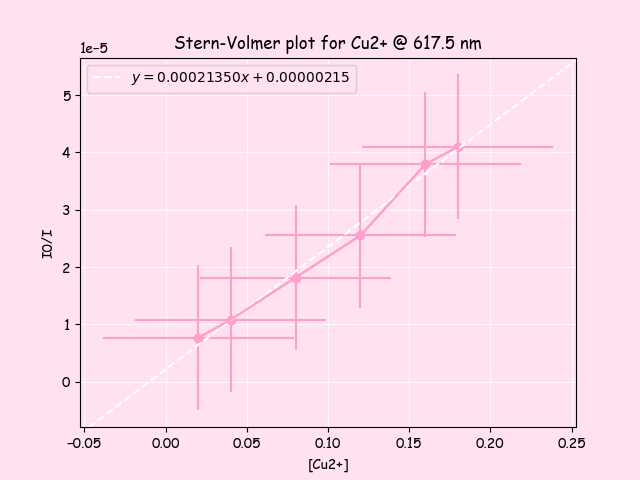
\includegraphics[width=\textwidth]{part1_q1_Cu.png}
         \caption{\ce{Cu^{2+}}}
         \label{fig:part1_q1_Cu}
     \end{subfigure}
     \caption{Stern-Volmer plots for luminescent quenching measurements}
     \label{fig:stern_volmers}
\end{figure}

Figure \ref{fig:stern_volmers} represents the following curve (eqn (6)) from lab manual\autocite{lab_manual}:
\begin{equation*}
    \frac{I_0}{I} = 1 + \frac{k_q}{k_d}[Q]
\end{equation*}

So $\frac{k_q}{k_d}$ is the slope of each curve. The slope of \ref{fig:part1_fe} is
\input{part1_q1_fe_slope.txt}at a wavelength of \input{part1_q1_fe_wl.txt}nm, and \ref{fig:part1_q1_Cu} is \input{part1_q1_cu_slope.txt}at a wavelength of \input{part1_q1_cu_wl.txt}nm.
PUT HOW U FOUND WAVELENGTH
\\
\textbf{Question 2}
\par From the lab manual\autocite{lab_manual}, $k_d = 1.7 \times 10^6\text {s}^{-1}$. Thus,
\begin{equation}
    k_q = \text{slope} \times k_d
    \label{eq:p1q2}
\end{equation}

\begin{equation*}
    \mathcolorbox{Lavender}{A = 0.21066718C_{\text{digested}} -0.0077607}
\end{equation*}


\subsubsection*{Discussion Questions}

\subsection{Part 2}





\end{document}